\chapter{Technische Umsetzung}
\section{Aufbau des Backends}
\section{Beschreibung der verwendeten Services}


\section{Beschreibung der verwendeten APIs}
\subsection{BoardGameGeek XML API }

Die BoardGameGeek XML API bietet eine Schnittstelle zum Zugriff auf eine Vielzahl von Informationen rund um Brettspiele,
die auf BoardGameGeek.com, einer umfangreichen Datenbank und Community für Brettspiel-Enthusiasten,
verfügbar sind. Diese API ermöglicht es Entwicklern druch verschiedene Endpoints auf Spielinformationen,
Benutzerkollektionen und Forendiskussionen zuzugreifen. Dabei zu beachten ist, dass die API die Antwort als XML-Format weitergibt. 
Da häufig mit JSON gearbeitet wird ist eine mögliche Umformung der Daten sinnvoll.

\large Suchfunktion

Eine der beiden Endpunkte ist die `/xmlapi/search`-Funktion bei der Nutzer als Input einem spezifischen Suchterm eingeben.
Als Ergebnis enthält man eine Liste an Brettspielen in XML Format, deren Namen oder Alias im Suchbegriff enthalten war.
Die detaillierte Antwort enthält folgende Informationen:
\begin{itemize}
    \item {objectId des Brettspiels}
    \item {Name des Brettspiels}
    \item {Erscheinungsjahr des Brettspiels}
\end{itemize}

Die reale Ausgabe für den fiktiven Suchterm ``Frika'' würde somit folgendes zurückgeben: 
\begin{figure}[h]
    \centering
    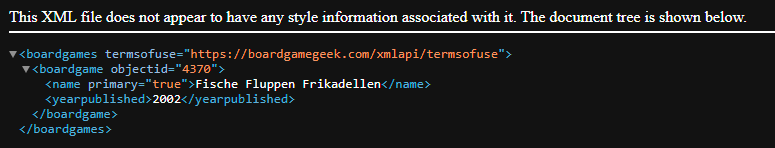
\includegraphics[width=1\textwidth]{graphics/Search_API.png}
    \caption{Ergebnis der `/xmlapi/search`-Funktion bei Suchterm Frika}
    \label{fig:Search_API}
\end{figure}

 \large Detaillierte Spielinformationen

Der andere Endpunkt ist die `/xmlapi/boardgame/<gameid>`-Funktion und dient dazu,
detaillierte Informationen zu einem Brettspiel zu erhalten. Nutzer könnten hier noch einige weitere Parameter mitgeben um spezifische Informationen zu erhalten, jedoch ist dies in unserem Projekt nicht notwendig, da die Ergebnisse schon detailliert genug sind.
Die gameId ist hierbei der Input, ist gleichzusetzen mit der objectId und kann aus des oben erhaltenen Ergebnisses der Suchfunktion entnommen werden.
% Reduzieren des Abstands zwischen den Punkten
\begingroup
\setlength{\itemsep}{-1pt} % Setzt den Abstand zwischen den Punkten auf 0pt
\setlength{\parskip}{-1pt} % Optional: Reduziert den Abstand zwischen Absätzen
\begin{itemize}
    \item objectId: String
    \item yearPublished: String
    \item minPlayers: String
    \item maxPlayers: String
    \item playingTime: String
    \item minPlayTime: String
    \item maxPlayTime: String
    \item age: String
    \item description: String
    \item name: Array (String)
    \item publisher: Array (String)
    \item averageWeight: String
    \item averageRating: String
    \item thumbnail: String (Link to picture source)
    \item usersRated: String
\end{itemize}
\endgroup

Es ist zu erkennen, dass der Name und der Publisher Arrays sind. Dies lässt sich darauf zurückführen, dass es mehrere Namen für dasselbe Spiel gibt (teilweise auch in anderen Sprachen) und mehrere Entwicklet beteiligt sein können.

\subsection{MongoDB API}

LUKAS TEIL 
\subsection{Verwendung der API im Projekt selbst}
\section{Anleitung zum Starten der Applikation}
